\section{demag\_gui.py usage and
tips}\label{demagux5fgui.py-usage-and-tips}

The demag\_gui program enables the display and analysis of paleomagnetic
demagnetization data. The software will display specimen level data
within the chosen directory as a Zijderveld plot, equal area plot and
intensity plot. Interpretations can be made to the data as least-squares
line or plane fits. These interpretations can then be exported within
MagIC pmag files.

\begin{figure}[htbp]
\centering
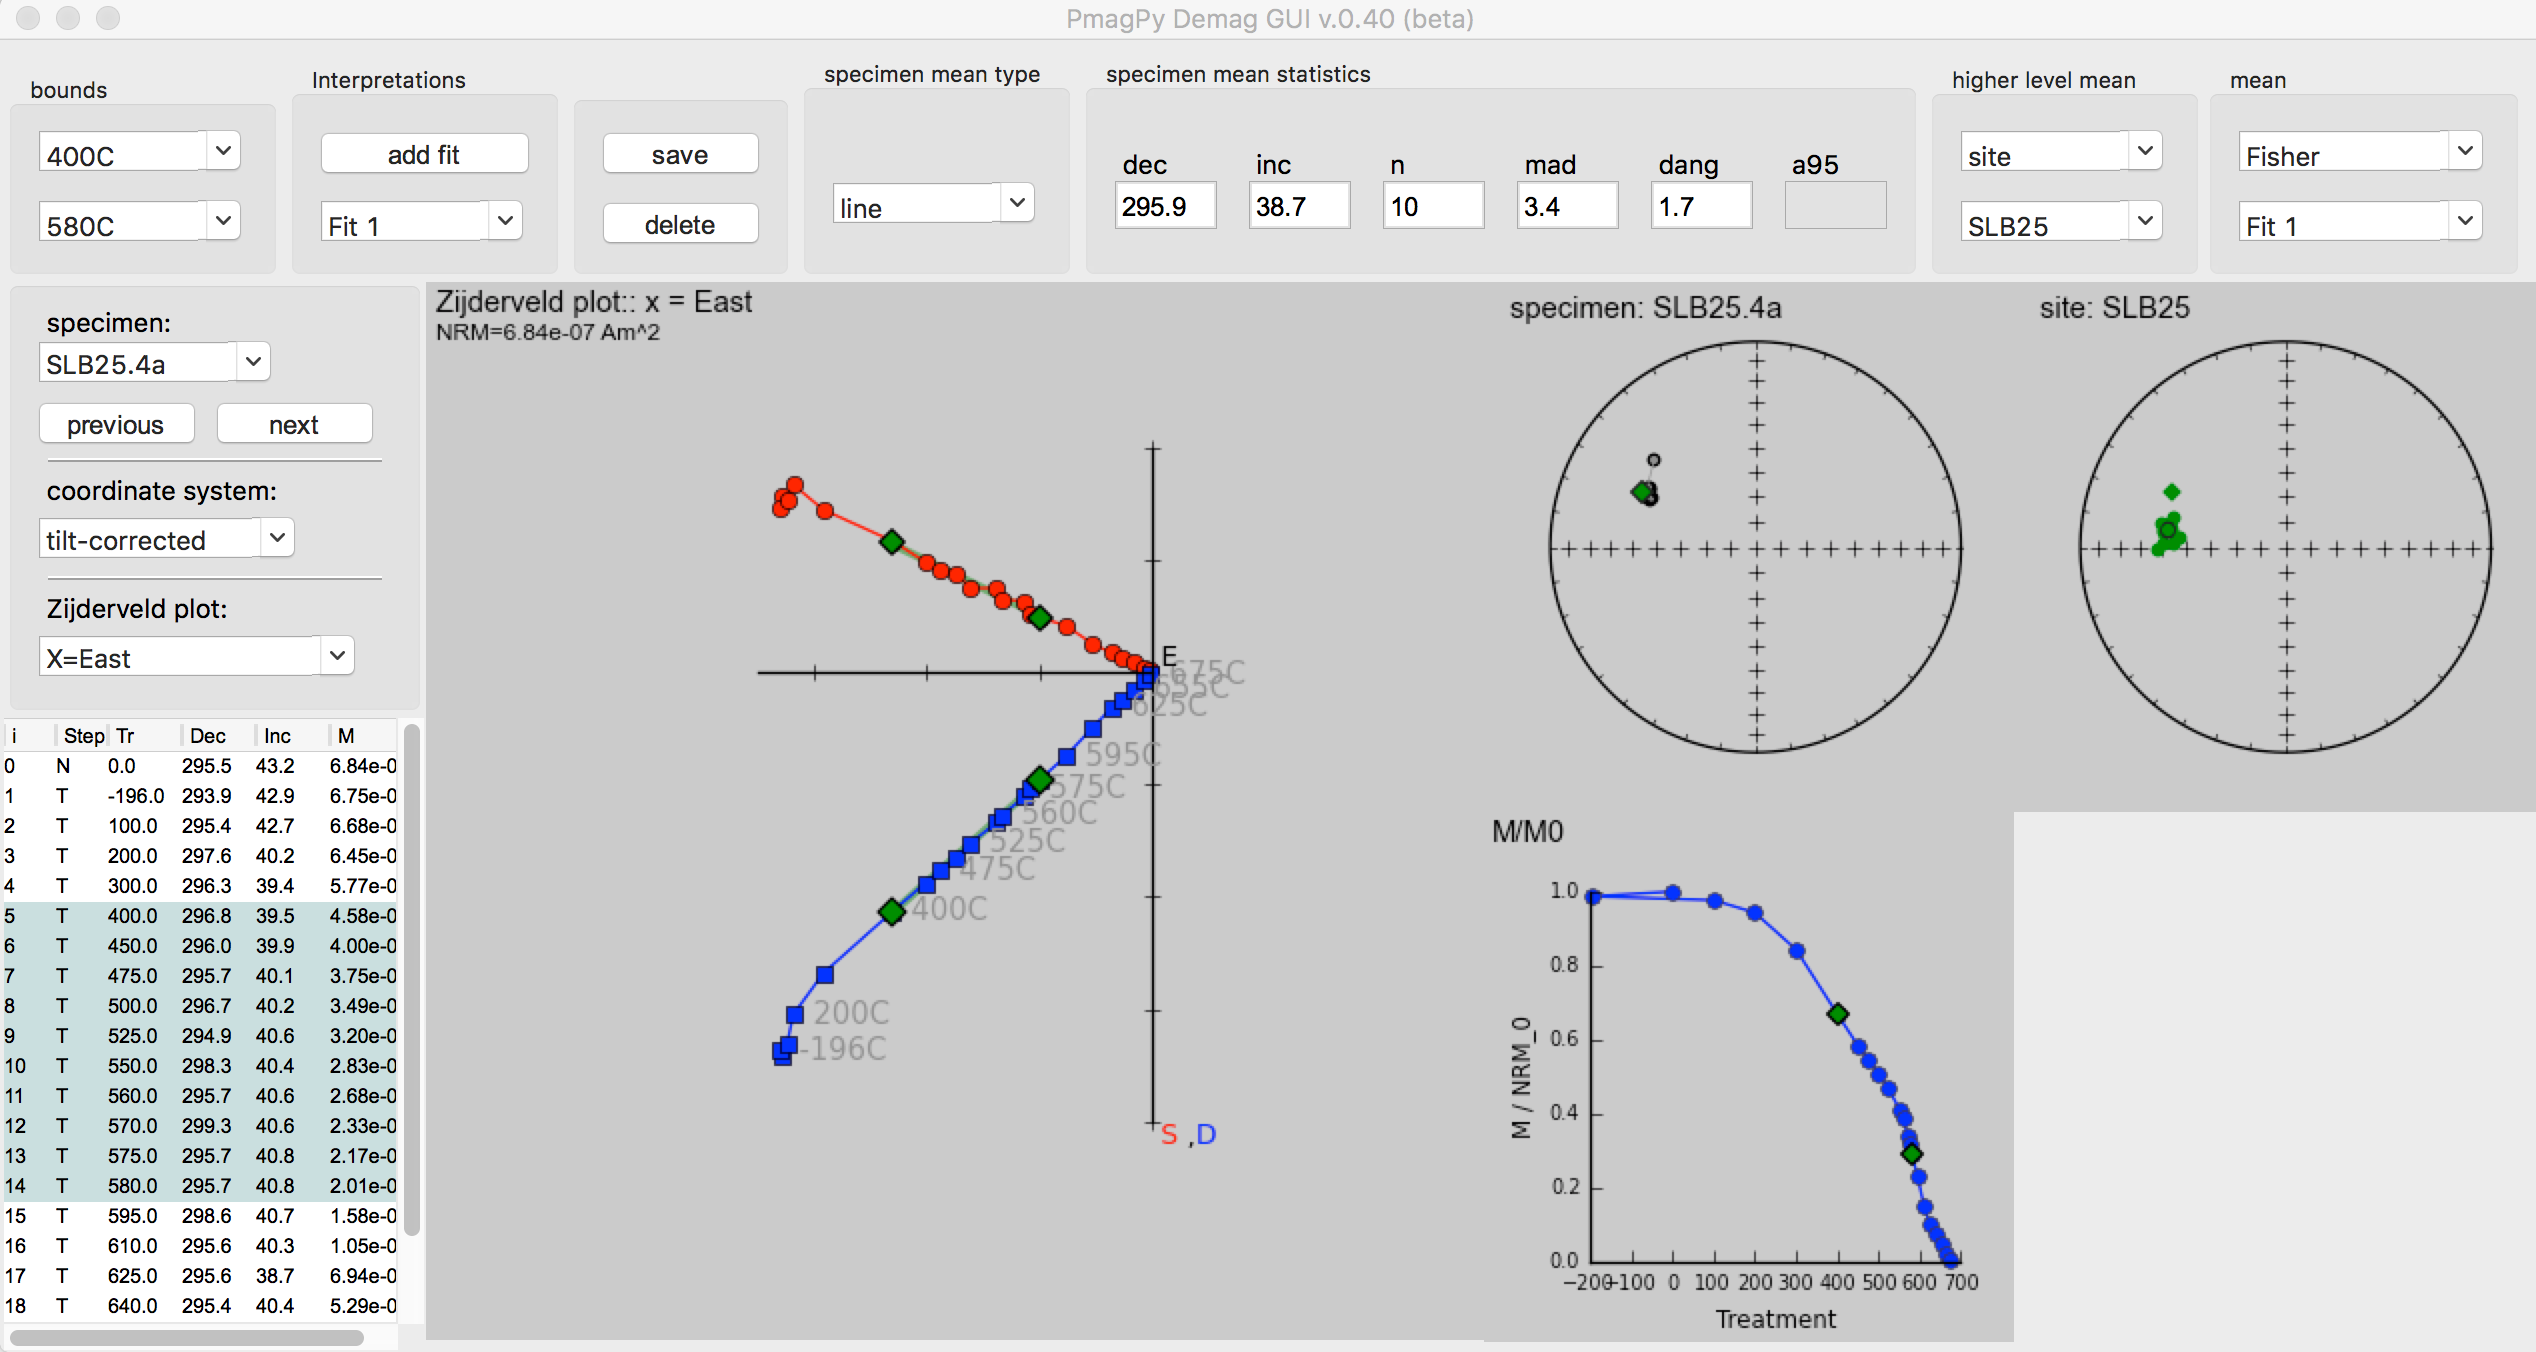
\includegraphics{./images/demag_gui.png}
\caption{}
\end{figure}

\subsection{Installing}\label{installing}

This program is part of the
\href{https://github.com/ltauxe/PmagPy}{PmagPy repository} which can be
downloaded or cloned from Github. To run demag\_gui.py it is necessary
to download and install a working version of
\href{https://www.python.org/downloads/}{python 2.7}, the latest version
of the GUI library
\href{http://www.wxpython.org/download.php}{wxpython}, and the basic
scientific libraries that are part of the
\href{http://www.scipy.org/install.html}{scipy project}. The easiest way
to get all that you need is to install the Enthought Canopy distribution
as described in the PmagPy cookbook:
http://earthref.org/PmagPy/cookbook/\#QQ2-1-2.

\subsection{Launching}\label{launching}

The best way to launch the demag\_gui application is through the
QuickMagIC app. If PmagPy has been added to your PATH you can type
QuickMagIC.py at the command line to launch it or you can navigate to
the directory containing it and type \texttt{python\ ./QuickMagIC.py}.
Within the QuickMagIC app, data can be converted from the format of a
particular lab into MagIC format so that it can be displayed and
analyzed within the demag\_gui. The program can be started by clicking
on the demag\_gui button in the QuickMagIC GUI, shown below.

\begin{figure}[htbp]
\centering
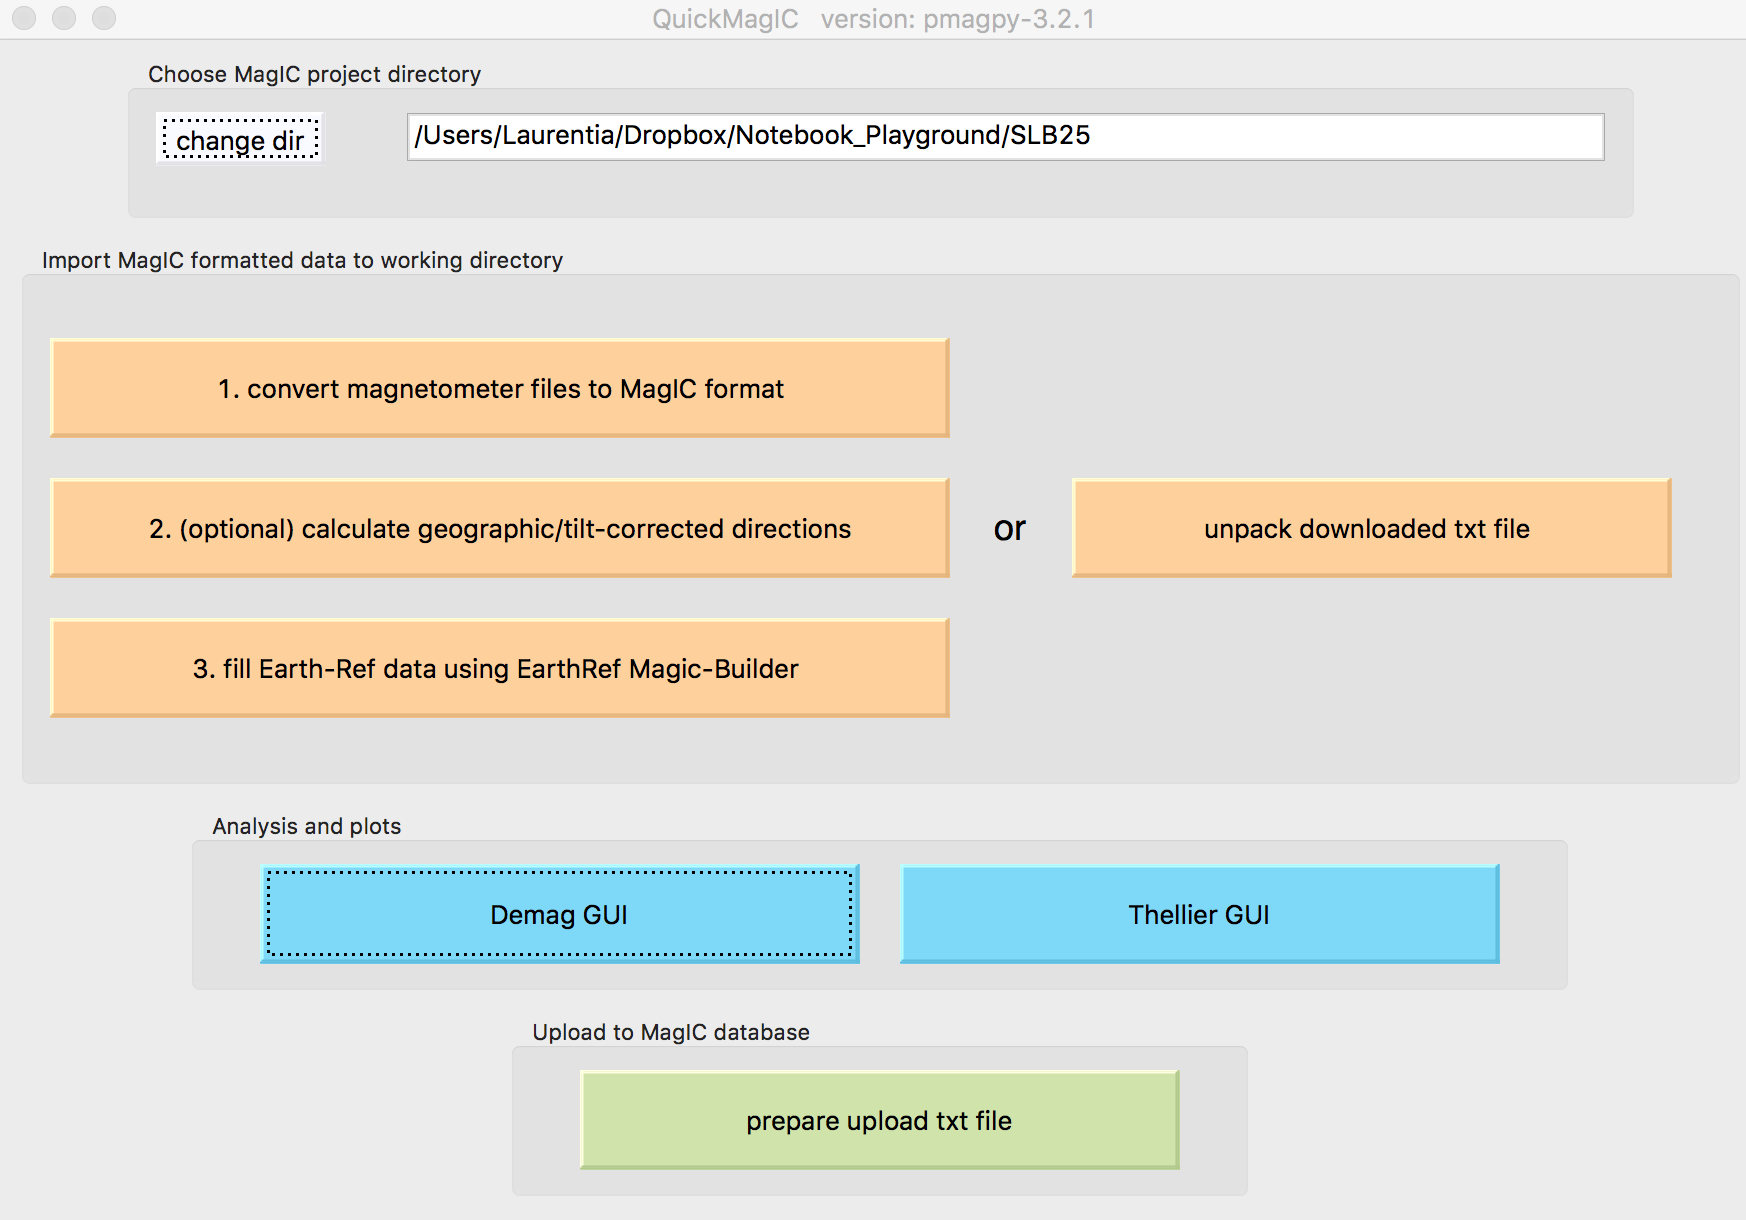
\includegraphics{./images/QuickMagicLauncher.png}
\caption{}
\end{figure}

Alternatively, the demag\_gui may be launched through the command line
by navigating to the directory containing demag\_gui.py and running it
with:

\begin{Shaded}
\begin{Highlighting}[]
\KeywordTok{python} \NormalTok{./demag_gui.py}
\end{Highlighting}
\end{Shaded}

Or if PmagPy has been added to your PATH you can simply type
demag\_gui.py at the command line. \textbf{Note:} on OSX it is
recommended to launch through the QuickMagIC program as on wxpython 2.9
the drop down boxes behave better when demag\_gui is launched this way.

\subsection{Interpretation of Specimen
Data}\label{interpretation-of-specimen-data}

\subsubsection{Adding Interpretations:}\label{adding-interpretations}

A least-squares fit to the measurement data can be added by clicking the
add fit button. Additionally, you can select the fit you would like to
edit or view by using the drop down box under the add fit button. Once
you have selected a fit, the shape of the end points of the selected fit
will turn to a diamond shape to distinguish them from the other data
points.\\
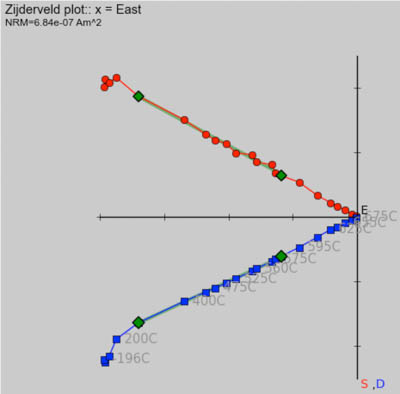
\includegraphics{./images/Fit.jpg}

Once the desired fit is selected, its bounds can be edited using the
drop-down boxes under the bounds header.
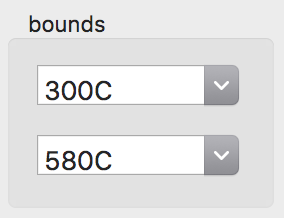
\includegraphics{./images/BoundsBox.png}

Alternatively, one can double-click the list of measurement steps on the
left to pick out the bounds for the interpretation. The included steps
in the currently selected interpretation are shown in highlighted in
blue on the measurement list and the measurements marked ``bad'' are
shown in yellow. \textbf{Note:} in case of duplicate measurements the
first \emph{good} measurement with the same treatment is used.\\
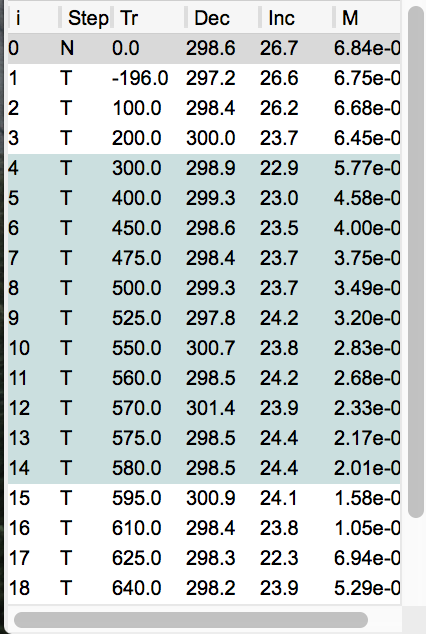
\includegraphics{./images/DataBox.png}

When first created, the fit will be given a generic name such as
\emph{Fit 1}. The name of the fit can be changed from the default by
typing into the drop down box containing fit name then pressing enter.
The default fit type is a least-squares line. You can choose different
fits such as a line anchored to the origin or a plane by using the drop
down menu under specimen mean type. Planes can be plotted as either
poles, full planes or partial planes. This display option can be changed
in the second drop-down menu under specimen mean type.
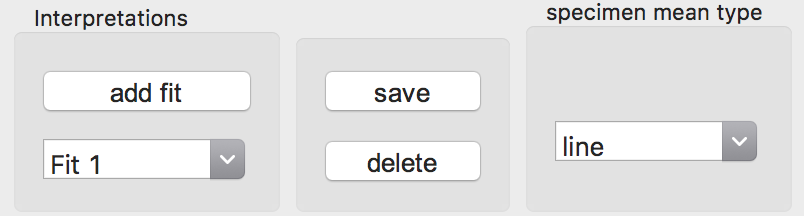
\includegraphics{./images/SpecimenMeanType.png}

The choice between coordinate systems (i.e.~specimen, geographic or
tilt-corrected) is available on the left above the list of steps. The
orientation of the Zijderveld projection can also be changed here.
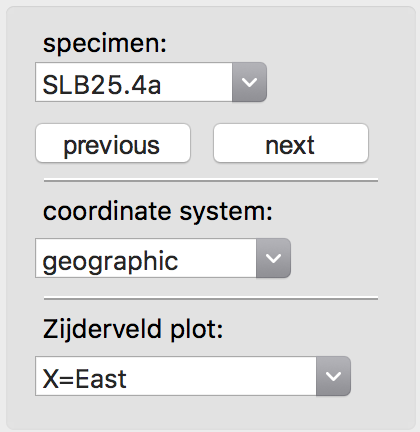
\includegraphics{./images/ProjectionChoice.png}

The properties of the currently selected fit to the data can be seen in
the upper center of the GUI in a box labeled specimen mean statistics.
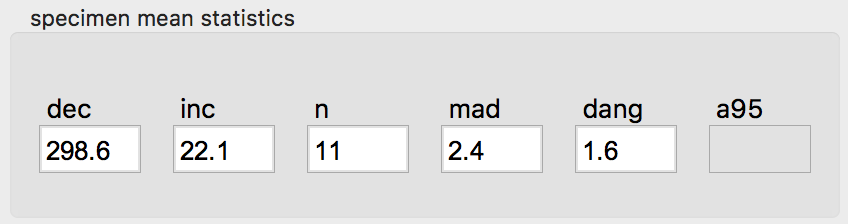
\includegraphics{./images/FitData.png}

\subsubsection{Flagging Bad Measurement
Data}\label{flagging-bad-measurement-data}

Due to flux jumps or other such errors, individual measurements should
sometime be excluded from interpretation. Such a measurements can be
flagged as ``bad'' by right-clicking them within the measurement list
and the measurement will then be highlighted in yellow. The
measurement\_flag in the magic\_measurements file will be change from
``g'' to ``b'' when a measurement is marked as ``bad'' and the step will
not be included in fits that are made to the data. Any measurement
marked as `bad' will be colored yellow in the step list and will be
shown as an empty rather than filled circle on the Zijdeveld, equal area
and M/M\_0 plots. To change a `bad' measurement back to being `good' one
can right click on it again. Upon doing so, the yellow highlighting will
go away, the data will be shown colored in within the plots and any fit
that spans that data point will be recalculated to include it.

Acceptance criteria can be set by using Analysis/``Acceptance
Criteria''/``Change Acceptance Criteria''. These criteria will be
written to a pmag\_criteria table.

\subsubsection{Plot Interface}\label{plot-interface}

The 4 plots that take up the majority of the center of the GUI are where
data and their interpretations are displayed. The Zijderveld and the 2
equal area plots are by default set to zoom when you left click and drag
your left mouse button you will zoom to the dragged out rectangle
(currently equal area plots do not draw this rectangle as you drag your
mouse, but still zoom). On the Zijderveld plot, it is possible to switch
between zoom and pan functionality by right clicking. Once in pan mode,
the mouse will turn into a hand allowing you then to click and move
around the plot. On both the Zijderveld and equal area plots if you wish
to return to the original plot simply click the middle mouse button to
return to home position. \textbf{Note:} in the absence of a middle mouse
button pressing both right and left mouse buttons at the same time works
on most laptops in the case of Macbooks clicking with two fingers should
work, and if using Apple's magic mouse we recommend you download the
\href{http://magicprefs.com/}{MagicPrefs} program which will allow you
to configure your mouse however you prefer. One the equal area plots you
can double click on an interpretation to switch the specimen and current
interpretation to the clicked interpretation.

\subsubsection{Saving Specimen
Interpretations}\label{saving-specimen-interpretations}

Once you have picked out your interpretations, you can save the session
data in two different ways: (1) as a .redo file which will allow you to
have the fits preserved to be view again with demag\_gui or (2) as MagIC
pmag tables to be uploaded to the MagIC database or otherwise processed.
In addition, you may save image files of the plots.

\paragraph{The .redo File:}\label{the-.redo-file}

You can use Analysis/``Save current interpretations to a redo file'' to
create this file type or you can just hit the save button next to add
fit. \textbf{Note:} this file type does \textbf{NOT} load previous
interpretations on start up you must go to the menu option
Analysis/``Import previous interpretations from a redo file'' to restore
your previous session.

\paragraph{The Pmag Tables:}\label{the-pmag-tables}

By going to the menu File/``Save MagIC pmag tables'' you can export your
interpretations made in Demag GUI to the MagIC pmag tables which can
then be used by other MagIC programs or uploaded to the MagIC database.
You can export any or all of the 3 coordinate systems upon selecting
this option and you may choose to save pmag\_samples, pmag\_sites, and
pmag\_results tables in addition to the pmag\_specimens table that is
output. If you choose to output additional information you will be
prompted by a pop up window for additional information. \textbf{Note:}
this save format loads on start up of the GUI immediately restoring your
session. Selection of this option will overwrite your demag\_gui.redo
file in the working directory.

\paragraph{Images of Plots:}\label{images-of-plots}

Select the menu option File/``Save plot''/``Save all plots'' to save all
plots. Alternatively, you can save any of the plots individually. If you
zoom on any of the plots the zoomed image will be saved not the
originally plotted image although the plot will redraw and reset the
zoom level.

\subsubsection{Deleting Specimen
Interpretations}\label{deleting-specimen-interpretations}

If you would like to delete a single interpretation, select the one you
wish to delete from the interpretation drop down menu and click delete.
Alternatively, if you wish to clear all interpretations you may go into
the interpretation editor located under the tools menu, select the fits
you wish to delete and click the ``delete selected'' button.\\

\subsection{Higher Level Plots and
Interpretation}\label{higher-level-plots-and-interpretation}

The set of drop down boxes to the right of the interpretation data are
there to determine what level you want to analyze in the higher level
analysis options include: site, sample, location, and study. The drop
down below this selects which of the available sites, samples, location,
or studies to display.

You can then select how to group your data by using the drop down menu
under the show header. You can select what kind of mean to take using
the first drop down under the mean header. Which interpretations to use
for the means can be selected under the second drop down menu.

The mean statistics for the chosen higher level mean are displayed in
the lower right of the GUI.

\subsubsection{Interpretation Editor}\label{interpretation-editor}

In order to more easily view and edit specimen interpretation data there
is a specimen interpretation editor which can be launched from the tools
menu. This panel details the fits made to the data and their parameters
from which you can select which interpretation to view by double
clicking on it. In the list, the currently selected interpretation is
highlighted blue as shown in the image below. You can mark
interpretations as bad which removes them from any Fisher means or other
high level means by right clicking on their entry in the list. All
interpretations marked bad are colored yellow in the list and marked as
a `x' on the plot. The specimen entry associated with this fit will be
given a bad (`b') flag within the pmag\_specimens table. Interpretations
can be highlighted by clicking on the list and holding the shift or
ctrl/command key to select multiple interpretations. Doing so allows you
to delete or alter the characteristics of multiple interpretations at
once without having to select each one in turn. This mass alteration is
allowable using the the Name/Color/Bounds boxes to input the changes and
then clicking the ``apply changes to highlighted fits'' button. You can
delete highlighted fits using the ``delete highlighted fits'' button.
The ``add fit'' button in the interpretation editor adds a fit to the
current specimen. In the case of interpreting large data sets, you can
reduce the number of items plotted on the equal area at the bottom of
the editor and the number of entries in the log by changing the display
settings. The equal area plot on the bottom works just like the higher
level equal area on the main Demag GUI panel allowing you to select
interpretations on it by double clicking and to zoom by clicking and
dragging.

\begin{figure}[htbp]
\centering
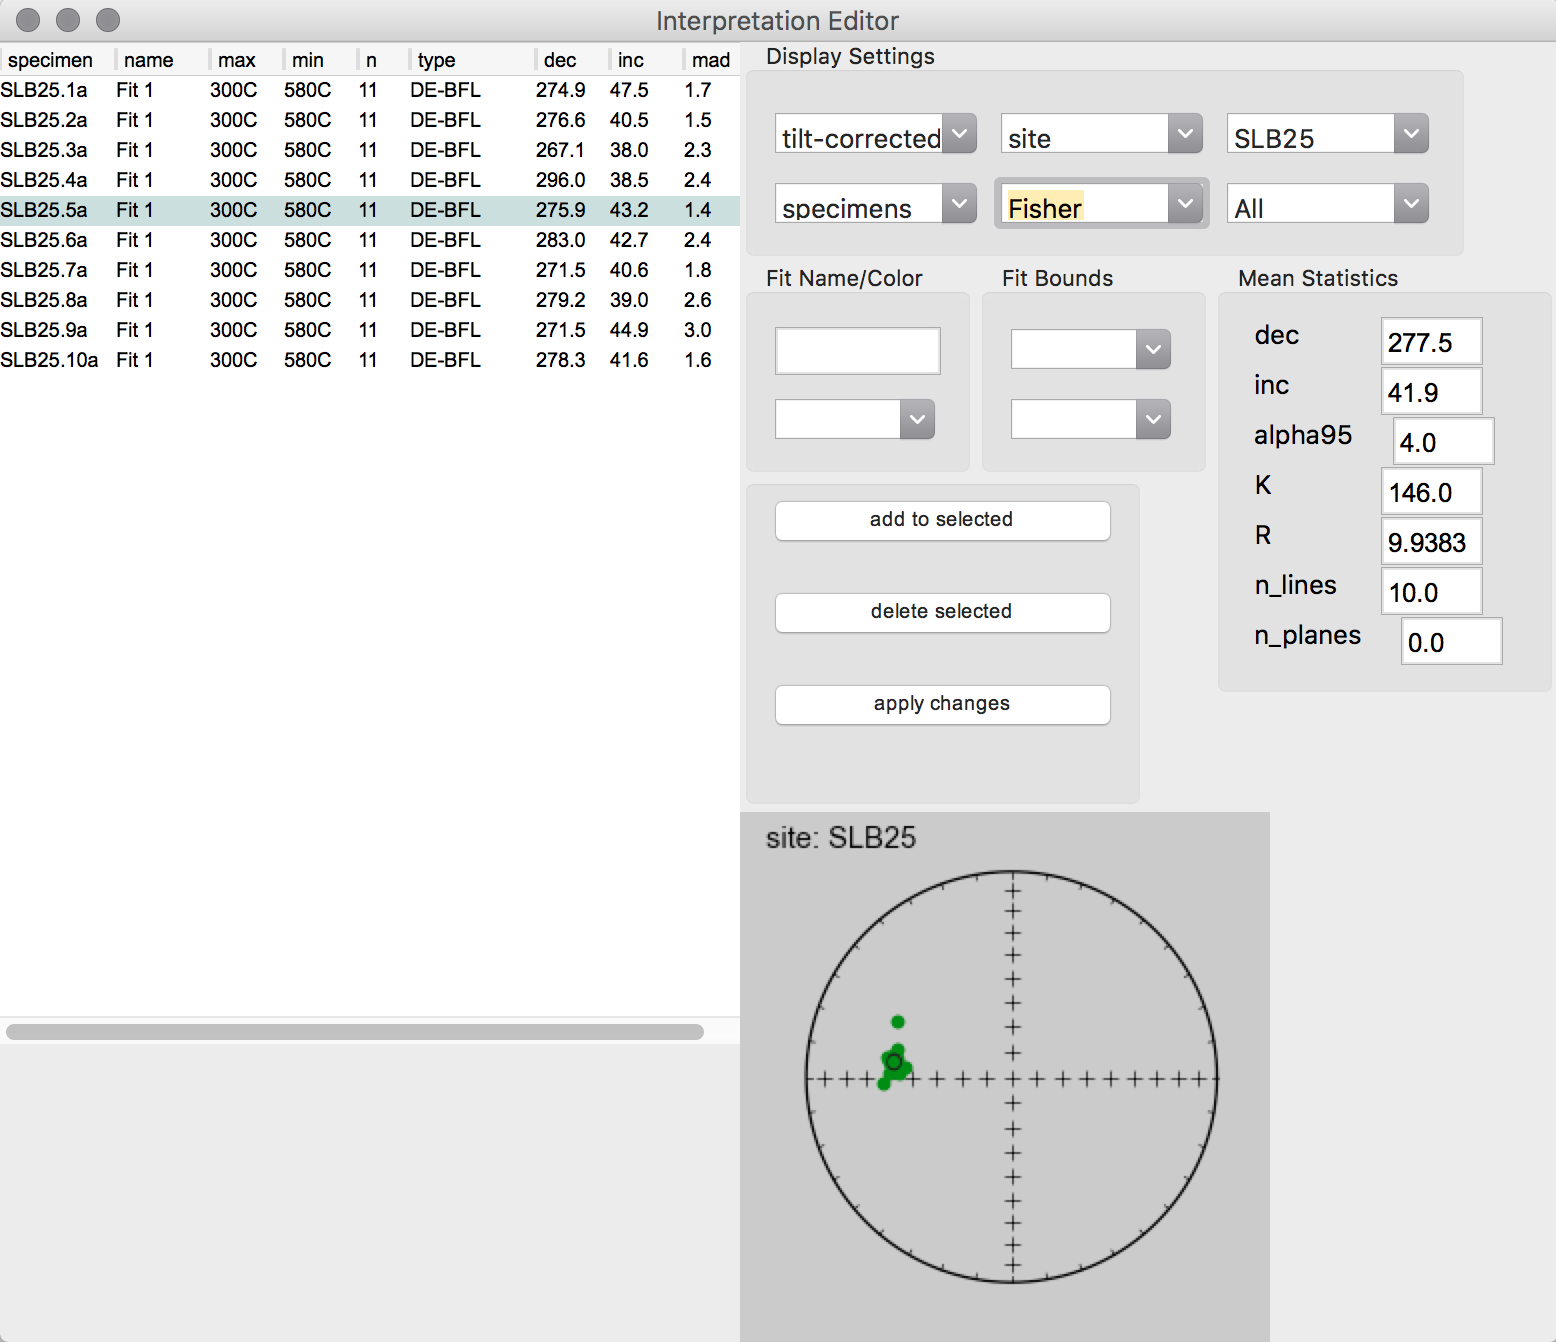
\includegraphics{./images/InterpEditor.png}
\caption{}
\end{figure}
